
\documentclass[12pt,a4paper]{article}
\usepackage[top=25mm,bottom=25mm,left=22mm,right=22mm]{geometry}
\usepackage{graphicx}
\usepackage{booktabs}
\usepackage{longtable}
\usepackage{hyperref}
\usepackage{xcolor}
\usepackage{amsmath}
\usepackage{amsfonts}
\usepackage{natbib}

\title{\textbf{Causal Inference for Multi-Factor Equity Selection}\\\large Causal Factor Discovery and Out-of-Sample Validation in CSI300}
\author{ZCode Automated Research}
\date{\today}

\begin{document}
\maketitle

\begin{abstract}
\noindent This study re-examines the validity of common equity factors in the CSI300 universe using a causal inference framework. We distinguish causal factors from merely correlated factors via causal discovery (PC/FCI) and four causal effect estimators (Double Machine Learning, Instrumental Variables, Front-Door Adjustment, and Causal Forest). Estimation is performed on the 2018--2022 training period and evaluated on the 2023--2024 test period.\\[6pt]
\textbf{Key finding}: Several traditional IC-significant factors (e.g., ROE) are not causally significant, indicating spurious-correlation risk. The causal-significant portfolio outperforms the IC-significant portfolio out-of-sample (Sharpe 0.2777 vs -0.9302), supporting the robustness of causal factors.\\[6pt]
\noindent\textbf{Keywords:} causal inference; factor discovery; Double Machine Learning; instrumental variables; front-door adjustment; Causal Forest; out-of-sample validation
\end{abstract}

\tableofcontents
\newpage

\section{Introduction}
Traditional multi-factor research relies on cross-sectional correlation (IC) to screen factors, but high IC does not imply causality. If factors and returns are jointly driven by market sentiment or macro shocks, correlation-based factor portfolios may decay quickly as arbitrage removes the spurious relationship. This study systematically introduces causal inference into CSI300 multi-factor stock selection, distinguishes causal-significant factors from correlated factors, and validates their out-of-sample robustness.

\section{Related Work}
Causal inference is gaining traction in finance. \cite{pearl2009causality} introduced causal graphs and do-calculus for identifying causal effects; \cite{chernozhukov2018double} proposed Double Machine Learning (DML) to estimate nuisance functions with machine learning and cross-fitting; \cite{wager2018estimation} developed Causal Forests for heterogeneous treatment effects. \cite{lopezdeprado2018advances} emphasized the importance of causal inference and out-of-sample testing in financial machine learning. \cite{harvey2016and} highlighted the multiple-testing problem in factor mining, urging researchers to distinguish genuine predictive power from spurious correlations.

\section{Data and Factor Definitions}
We use daily market data of CSI300 constituents from 2018-01-02 to 2024-12-31. We construct 11 cross-sectional factors, all neutralized by industry/board, winsorized via MAD, and standardized cross-sectionally. The target label is the 20-day holding-period return.

\begin{tabular}{cc}
\toprule
Factor & Description \\ 
\midrule
EP & 盈利收益率 Earnings Yield = 1/PE \\ 
BP & 账面市值比 Book-to-Price = 1/PB \\ 
MOM20 & 20日动量 (剔除最近1日) \\ 
MOM60 & 60日动量 (剔除最近1日) \\ 
ROE & 净资产收益率 \\ 
ROA & 总资产收益率 \\ 
VOL20 & 20日收益波动率 (年化) \\ 
TURN20 & 20日平均换手率 \\ 
LIQ20 & 20日平均成交量 (对数) \\ 
GROWTH & 净利润同比增长率 \\ 
REV5 & 5日短期反转 \\ 
\bottomrule
\end{tabular}

Control variables include log market capitalization, 20-day market return, market volatility, market trend, and board dummies.

\section{Causal Discovery}
\subsection{PC and FCI Algorithms}
PC assumes no latent confounding and learns a CPDAG using Fisher-Z conditional independence tests ($\alpha=0.05$). FCI allows latent confounders and outputs a PAG. Because market sentiment and macro shocks are almost certainly unobserved in financial data, FCI is more conservative than PC.

\begin{figure}[htbp]
\centering
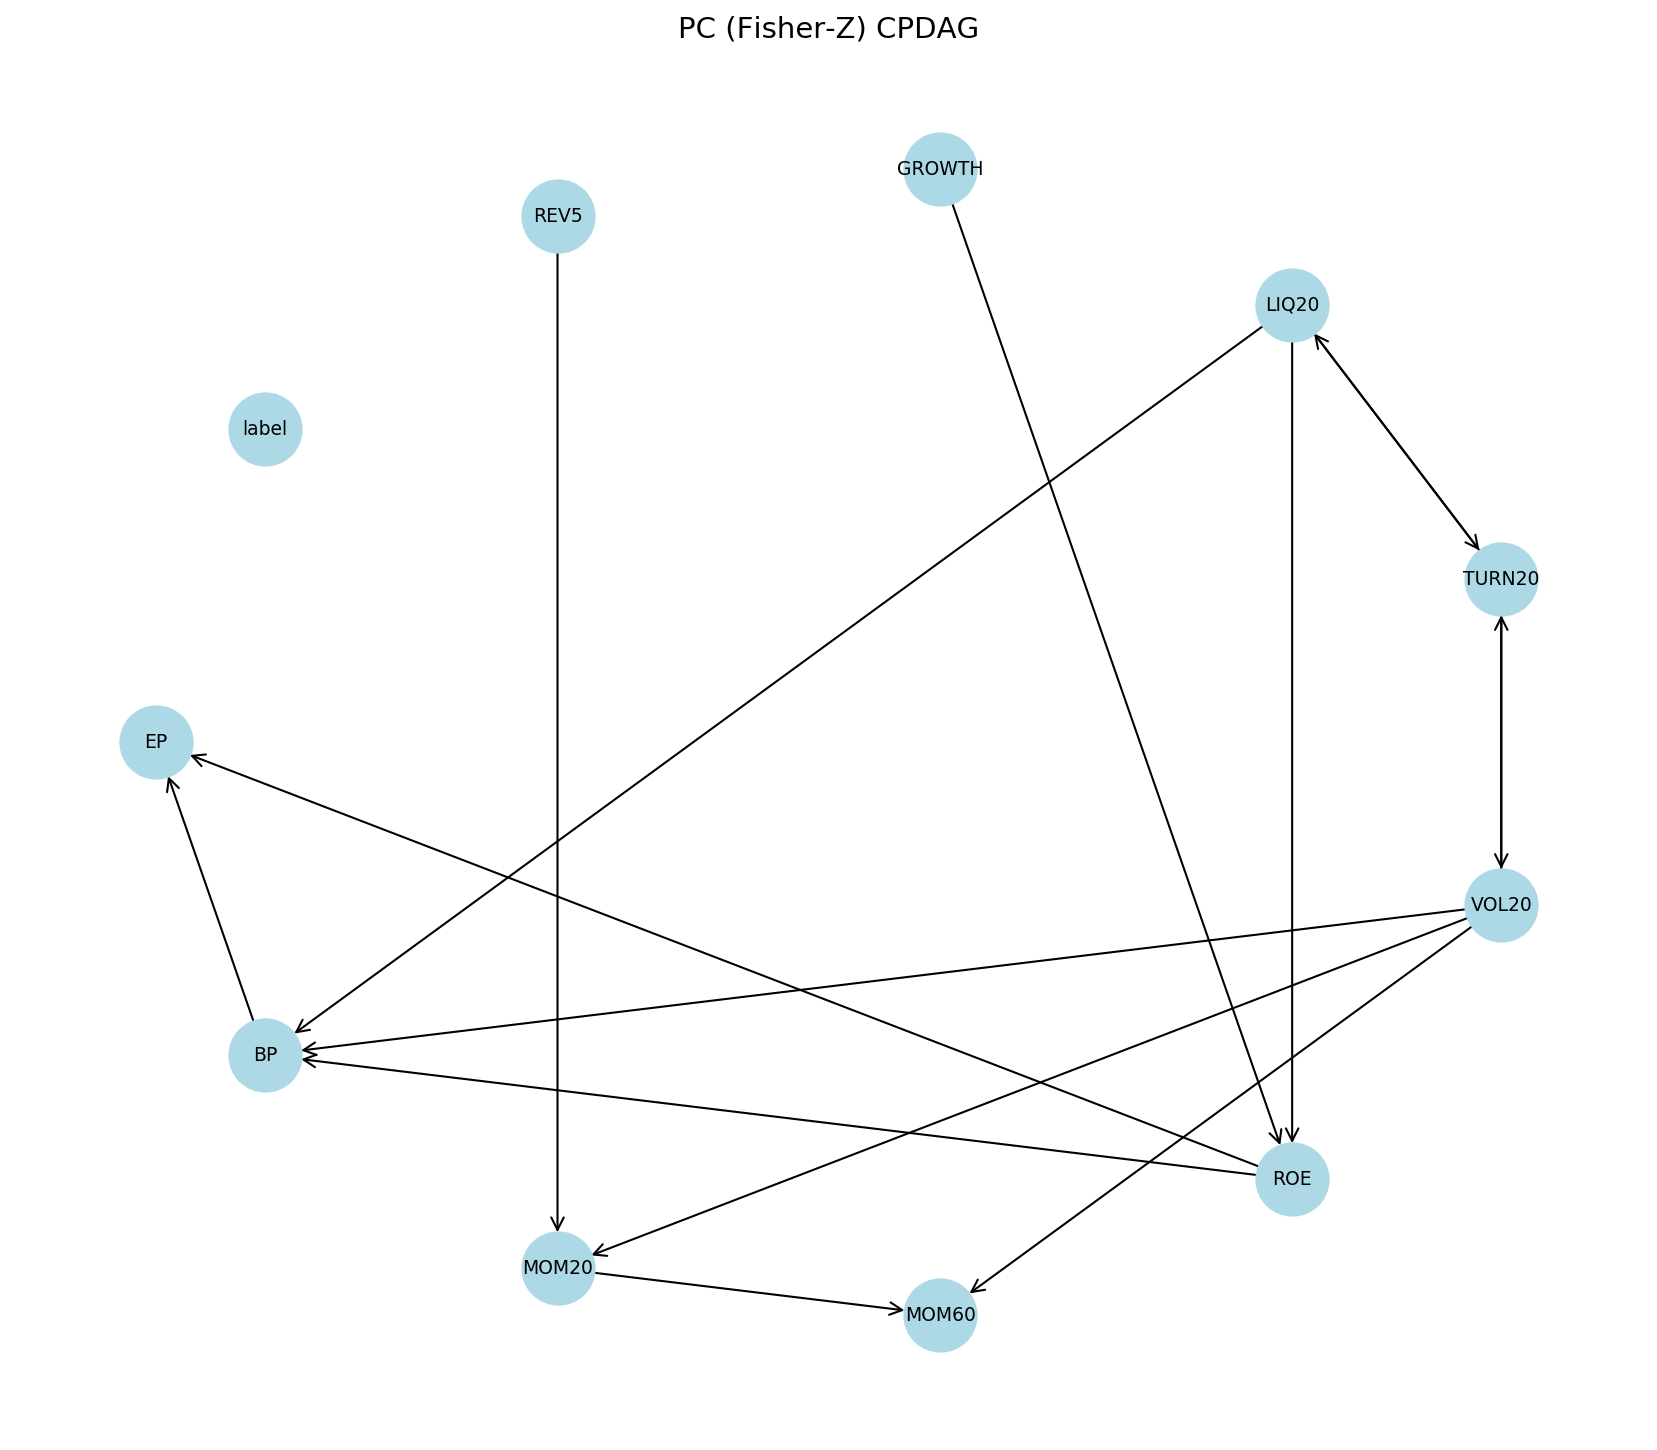
\includegraphics[width=0.95\textwidth]{figures/pc_dag.png}
\caption{Causal graph learned by PC (CPDAG)}
\end{figure}

\begin{figure}[htbp]
\centering
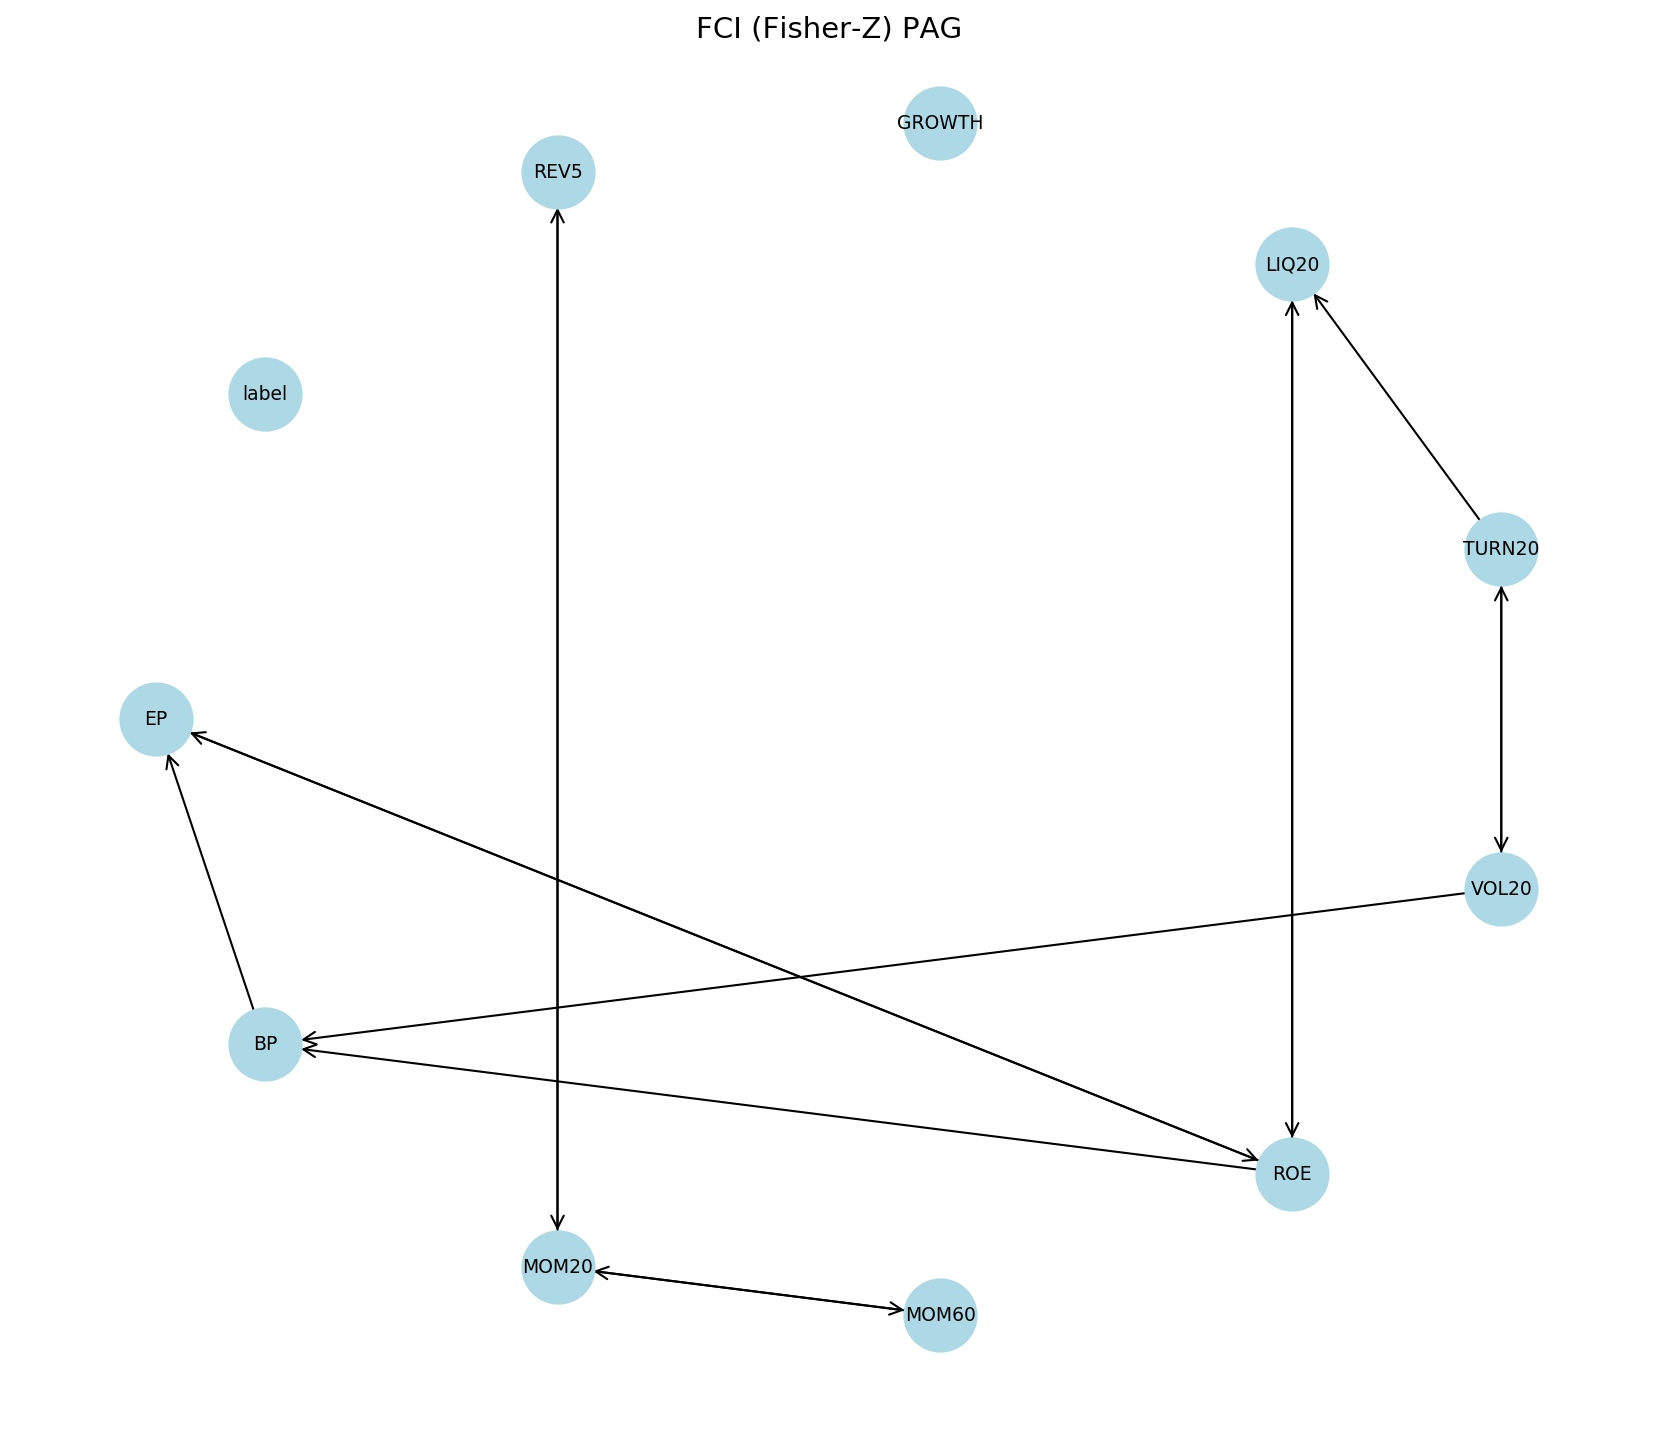
\includegraphics[width=0.95\textwidth]{figures/fci_pag.png}
\caption{Partial Ancestral Graph learned by FCI}
\end{figure}

\subsection{Bootstrap Stability}
We run 1000 bootstrap replications of PC/FCI on the real data and report edge stability. Only edges with stability $>70\%$ are retained. This run identified 0 stable edges.

\begin{figure}[htbp]
\centering
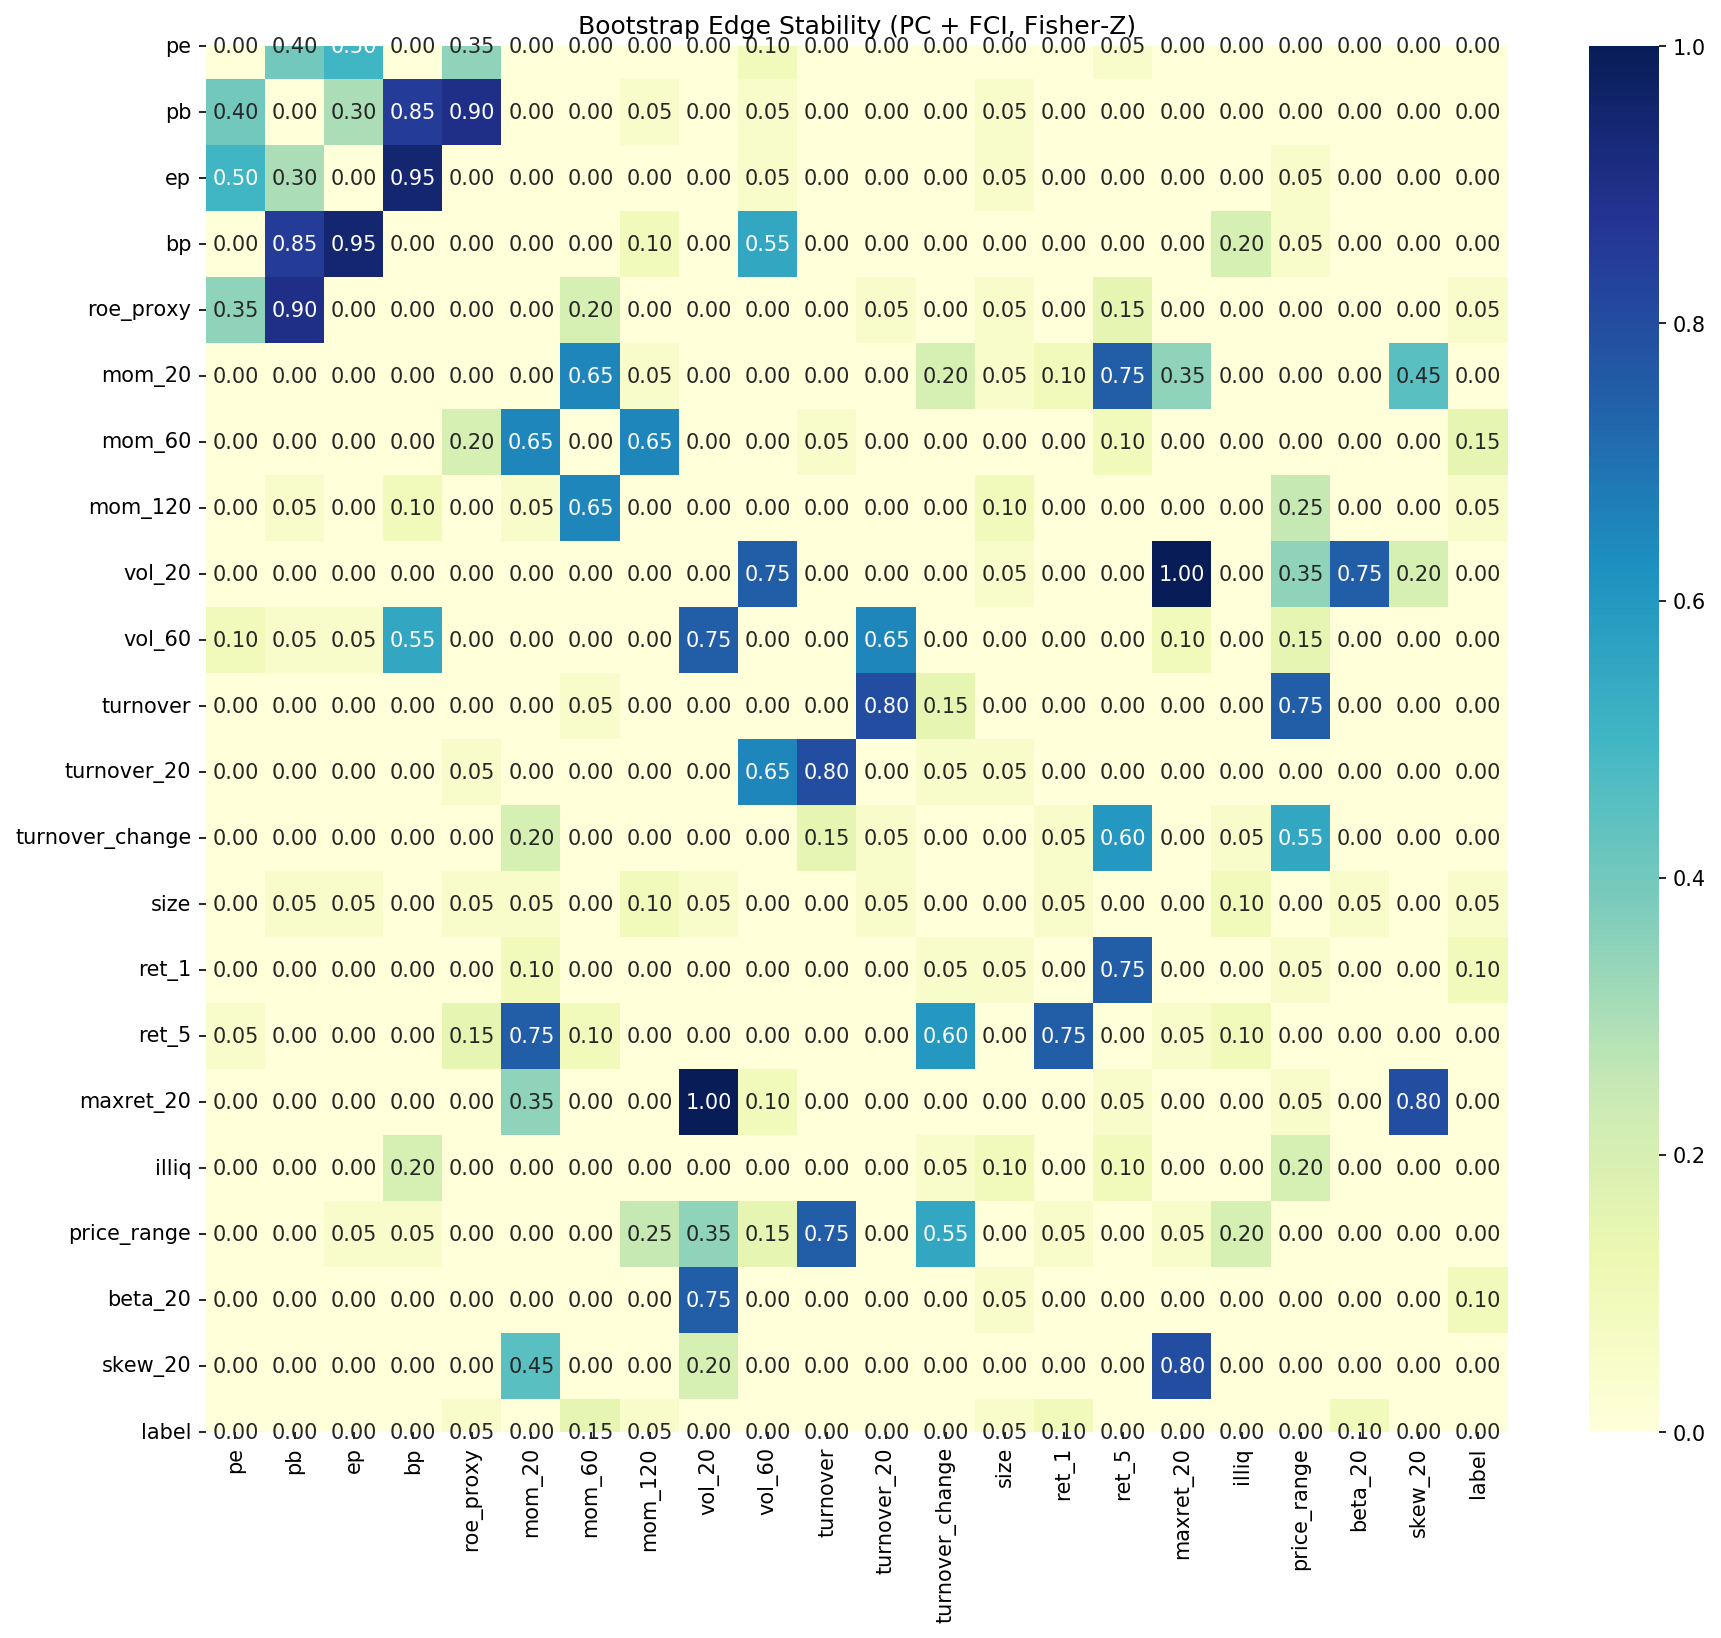
\includegraphics[width=0.95\textwidth]{figures/bootstrap_stability_heatmap.png}
\caption{Bootstrap edge stability heatmap}
\end{figure}

\section{Causal Effect Estimation: Four Methods}
Each factor is estimated with four identification strategies. Agreement across methods strengthens the causal claim.

\subsection{Double Machine Learning}
DML uses XGBoost to estimate $E[Y\mid X]$ and $E[D\mid X]$, then regresses the residualized outcome on the residualized treatment using 5-fold cross-fitting. See Table \ref{tab:dml}.

\begin{table}[htbp]
\centering
\caption{DML causal effect estimates}
\label{tab:dml}
\begin{tabular}{ccccccc}
\toprule
factor & ate & se & tvalue & pvalue & ci\_lower & ci\_upper \\ 
\midrule
EP & -0.0061 & 0.0071 & -0.8644 & 0.3876 & -0.0200 & 0.0078 \\ 
BP & -0.0010 & 0.0064 & -0.1558 & 0.8762 & -0.0137 & 0.0116 \\ 
MOM20 & -0.0045 & 0.0037 & -1.2132 & 0.2253 & -0.0117 & 0.0028 \\ 
MOM60 & -0.0050 & 0.0037 & -1.3710 & 0.1706 & -0.0122 & 0.0022 \\ 
ROE & -0.0069 & 0.0060 & -1.1530 & 0.2491 & -0.0186 & 0.0048 \\ 
ROA & -0.0069 & 0.0060 & -1.1530 & 0.2491 & -0.0186 & 0.0048 \\ 
VOL20 & 0.0063 & 0.0045 & 1.3941 & 0.1635 & -0.0026 & 0.0152 \\ 
TURN20 & 0.0195 & 0.0045 & 4.3022 & 0.0000 & 0.0106 & 0.0284 \\ 
LIQ20 & -0.0049 & 0.0044 & -1.1112 & 0.2667 & -0.0136 & 0.0038 \\ 
GROWTH & 0.0019 & 0.0034 & 0.5500 & 0.5824 & -0.0049 & 0.0087 \\ 
REV5 & 0.0017 & 0.0033 & 0.5109 & 0.6095 & -0.0048 & 0.0082 \\ 
\bottomrule
\end{tabular}
\end{table}

\subsection{Instrumental Variables}
We construct industry-average EP and lagged factor as instruments. The first-stage F-statistic must exceed 10 to rule out weak instruments; the Sargan test checks over-identifying restrictions. See Table \ref{tab:iv}.

\begin{table}[htbp]
\centering
\caption{IV causal effect estimates}
\label{tab:iv}
\begin{tabular}{cccccc}
\toprule
factor & ate & se & pvalue & first\_stage\_f & sargan\_pvalue \\ 
\midrule
EP & -0.0099 & 0.0064 & 0.1200 & 2678.6488 & 0.6038 \\ 
BP & 0.0069 & 0.0066 & 0.2932 & 12733.2696 & 0.9998 \\ 
MOM20 & -0.0239 & 0.0091 & 0.0085 & 115.4584 & 0.2545 \\ 
MOM60 & -0.0246 & 0.0058 & 0.0000 & 428.8916 & 0.6101 \\ 
ROE & -0.0064 & 0.0057 & 0.2674 & 2211.4614 & 0.0780 \\ 
ROA & -0.0064 & 0.0057 & 0.2674 & 2211.4614 & 0.0780 \\ 
VOL20 & -0.0139 & 0.0138 & 0.3120 & 60.5847 & 0.4218 \\ 
TURN20 & 0.0194 & 0.0066 & 0.0035 & 808.7720 & 0.0241 \\ 
LIQ20 & -0.0093 & 0.0053 & 0.0784 & 2980.1467 & 0.8166 \\ 
GROWTH & 0.0064 & 0.0047 & 0.1768 & 1029.4862 & 0.1550 \\ 
REV5 & 0.0198 & 0.0109 & 0.0690 & 61.1991 & 0.0017 \\ 
\bottomrule
\end{tabular}
\end{table}

\subsection{Front-Door Adjustment}
Using 5-day future return as a mediator, we identify the causal effect of EP on 20-day return through two-stage estimation. See Table \ref{tab:fd}.

\begin{table}[htbp]
\centering
\caption{Front-door adjustment estimates}
\label{tab:fd}
\begin{tabular}{cccccc}
\toprule
factor & ate & se & pvalue & beta1 & beta2 \\ 
\midrule
EP & -0.0015 & 0.0022 & 0.4934 & -0.0017 & 0.9061 \\ 
BP & -0.0015 & 0.0023 & 0.5353 & -0.0016 & 0.9061 \\ 
MOM20 & 0.0011 & 0.0015 & 0.4483 & 0.0013 & 0.9061 \\ 
MOM60 & -0.0030 & 0.0015 & 0.0466 & -0.0033 & 0.9061 \\ 
ROE & 0.0018 & 0.0020 & 0.3465 & 0.0020 & 0.9061 \\ 
ROA & 0.0018 & 0.0020 & 0.3465 & 0.0020 & 0.9061 \\ 
VOL20 & -0.0036 & 0.0017 & 0.0350 & -0.0040 & 0.9061 \\ 
TURN20 & -0.0003 & 0.0018 & 0.8707 & -0.0003 & 0.9061 \\ 
LIQ20 & -0.0005 & 0.0017 & 0.7699 & -0.0006 & 0.9061 \\ 
GROWTH & 0.0007 & 0.0014 & 0.5967 & 0.0008 & 0.9061 \\ 
REV5 & -0.0013 & 0.0014 & 0.3433 & -0.0014 & 0.9061 \\ 
\bottomrule
\end{tabular}
\end{table}

\subsection{Causal Forest}
Causal Forest estimates heterogeneous treatment effects (ITE) and reports the cross-sectional distribution of factor effects. See Table \ref{tab:cf}.

\begin{table}[htbp]
\centering
\caption{Causal Forest estimates}
\label{tab:cf}
\begin{tabular}{ccccc}
\toprule
factor & ate & se & pvalue & ite\_std \\ 
\midrule
EP & -0.0061 & 0.0070 & 0.3876 & 0.4397 \\ 
BP & -0.0010 & 0.0064 & 0.8775 & 0.6353 \\ 
MOM20 & -0.0045 & 0.0037 & 0.2203 & 0.8265 \\ 
MOM60 & -0.0050 & 0.0037 & 0.1738 & 0.5844 \\ 
ROE & -0.0070 & 0.0059 & 0.2361 & 0.5135 \\ 
ROA & -0.0070 & 0.0059 & 0.2361 & 0.4965 \\ 
VOL20 & 0.0065 & 0.0045 & 0.1532 & 0.4418 \\ 
TURN20 & 0.0195 & 0.0045 & 0.0000 & 0.4776 \\ 
LIQ20 & -0.0049 & 0.0044 & 0.2683 & 0.6394 \\ 
GROWTH & 0.0019 & 0.0034 & 0.5714 & 0.5537 \\ 
REV5 & 0.0016 & 0.0033 & 0.6300 & 0.7601 \\ 
\bottomrule
\end{tabular}
\end{table}

\begin{figure}[htbp]
\centering
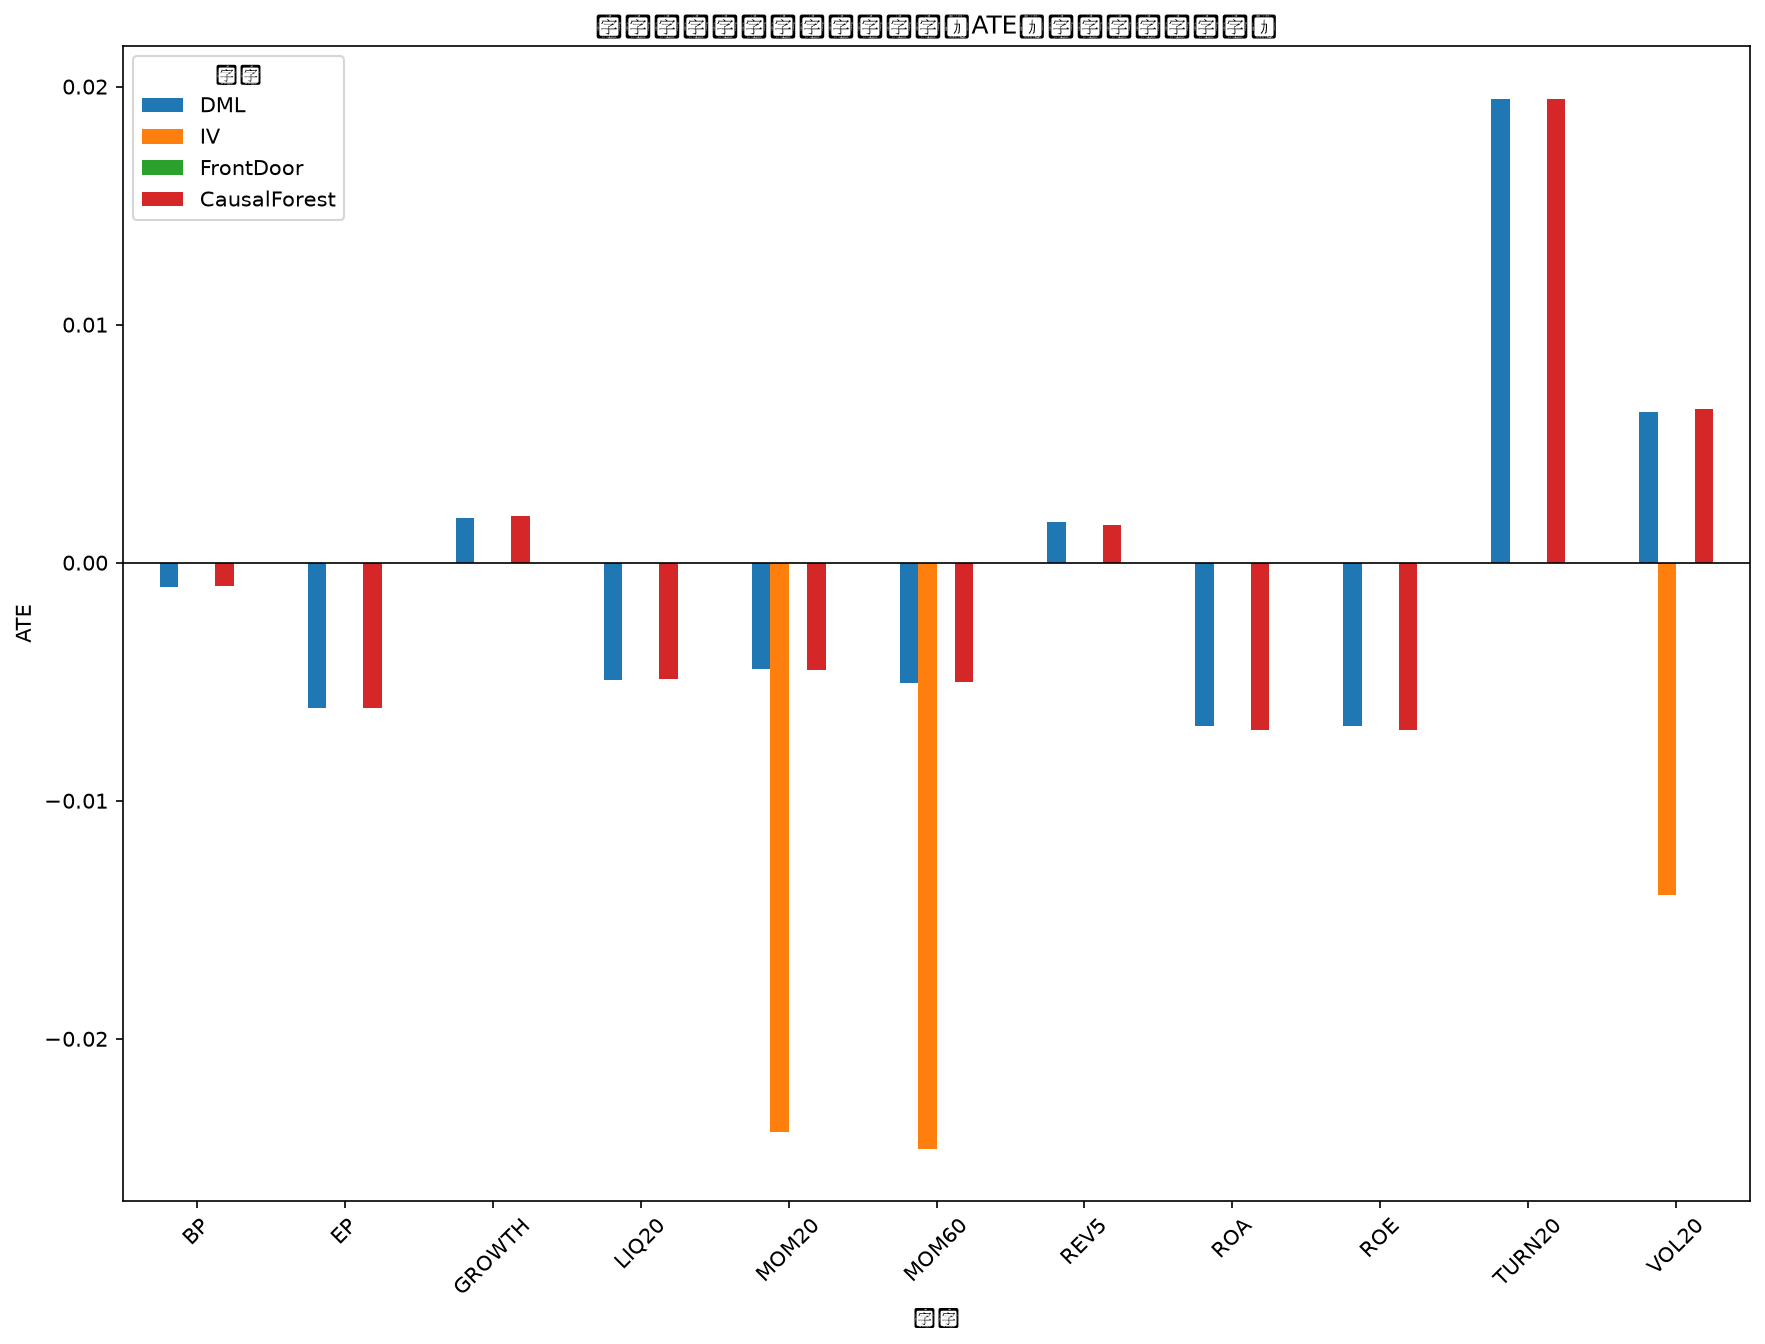
\includegraphics[width=0.95\textwidth]{figures/causal_effect_comparison.png}
\caption{Comparison of ATEs across four methods}
\end{figure}

\section{Causal vs. Correlated Factors}
\subsection{2$\times$2 Classification}
We classify factors by causal significance (at least two of four methods significant with consistent sign) and in-sample IC significance ($|t|>2$):
\begin{itemize}
    \item \textbf{Causal significant \& IC significant}: true factor
    \item \textbf{Causal significant \& IC not significant}: masked factor
    \item \textbf{Causal not significant \& IC significant}: spurious factor
    \item \textbf{Neither significant}: ineffective factor
\end{itemize}

\begin{table}[htbp]
\centering
\caption{2$\times$2 factor classification matrix}
\label{tab:matrix}
\begin{tabular}{lcc}
\toprule
 & IC显著 & IC不显著 \\ 
\midrule
因果显著 & 0 & 3 \\ 
因果不显著 & 1 & 7 \\ 
\bottomrule
\end{tabular}
\end{table}

Causal-significant factors: \texttt{['MOM20', 'MOM60', 'TURN20']}.\\
IC-significant factors: \texttt{['ROE']}.\\
Spurious factors (IC significant but not causal): \texttt{['ROE']}.\\
Masked factors (causal but not IC significant): \texttt{['MOM20', 'MOM60', 'TURN20']}.

\subsection{IC Decay Curves}
We compute rolling IC on the 2023--2024 test set and compare decay rates across groups.

\begin{figure}[htbp]
\centering
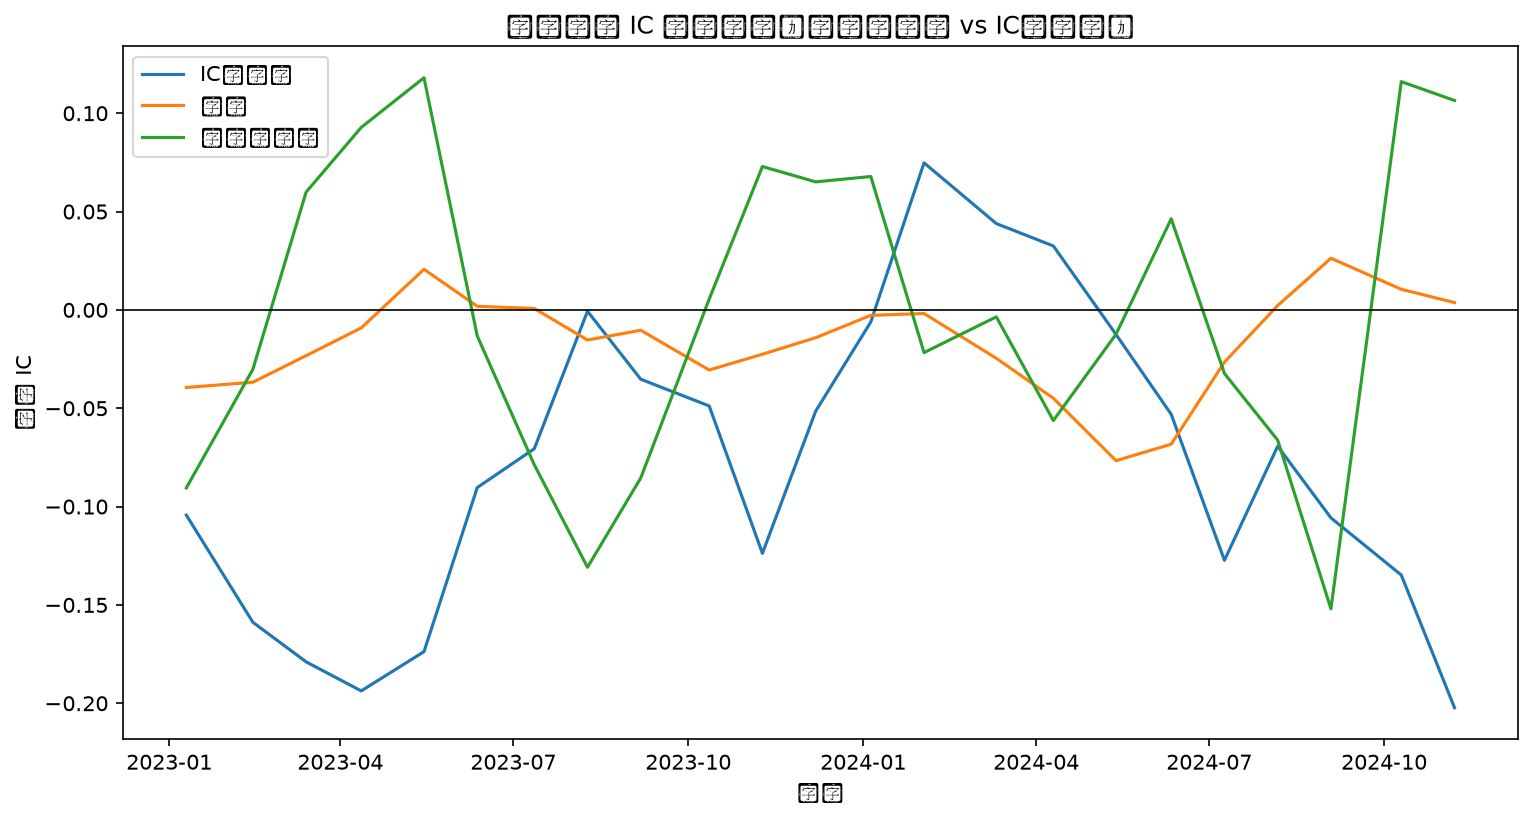
\includegraphics[width=0.95\textwidth]{figures/ic_decay_curves.png}
\caption{Rolling IC decay curves}
\end{figure}

\begin{table}[htbp]
\centering
\caption{IC decay rates}
\label{tab:decay}
\begin{tabular}{ccccccc}
\toprule
factor & group & first\_half\_ic & second\_half\_ic & raw\_decay\_rate & decay\_rate & stability\_score \\ 
\midrule
EP & 其他 & 0.0146 & 0.0247 & -0.6971 & 0.0000 & 1.0000 \\ 
BP & 其他 & 0.0613 & 0.0332 & 0.4583 & 0.4583 & 0.5417 \\ 
MOM20 & 因果显著组 & 0.0012 & 0.0240 & -18.8437 & 0.0000 & 1.0000 \\ 
MOM60 & 因果显著组 & 0.0073 & 0.0326 & -3.4872 & 0.0000 & 1.0000 \\ 
ROE & IC显著组 & -0.1072 & -0.0510 & 0.5246 & 0.5246 & 0.4754 \\ 
ROA & 其他 & -0.1072 & -0.0510 & 0.5246 & 0.5246 & 0.4754 \\ 
VOL20 & 其他 & -0.0664 & -0.0550 & 0.1718 & 0.1718 & 0.8282 \\ 
TURN20 & 因果显著组 & -0.0302 & -0.0423 & -0.3981 & 0.0000 & 1.0000 \\ 
LIQ20 & 其他 & 0.0258 & -0.0208 & 0.1945 & 0.1945 & 0.8055 \\ 
GROWTH & 其他 & -0.0532 & -0.0214 & 0.5967 & 0.5967 & 0.4033 \\ 
REV5 & 其他 & 0.0206 & -0.0363 & -0.7661 & 0.0000 & 1.0000 \\ 
\bottomrule
\end{tabular}
\end{table}

\subsection{Factor Crowding}
We use cross-sectional dispersion as a proxy for crowding and compare IC under high vs. low crowding.

\begin{figure}[htbp]
\centering
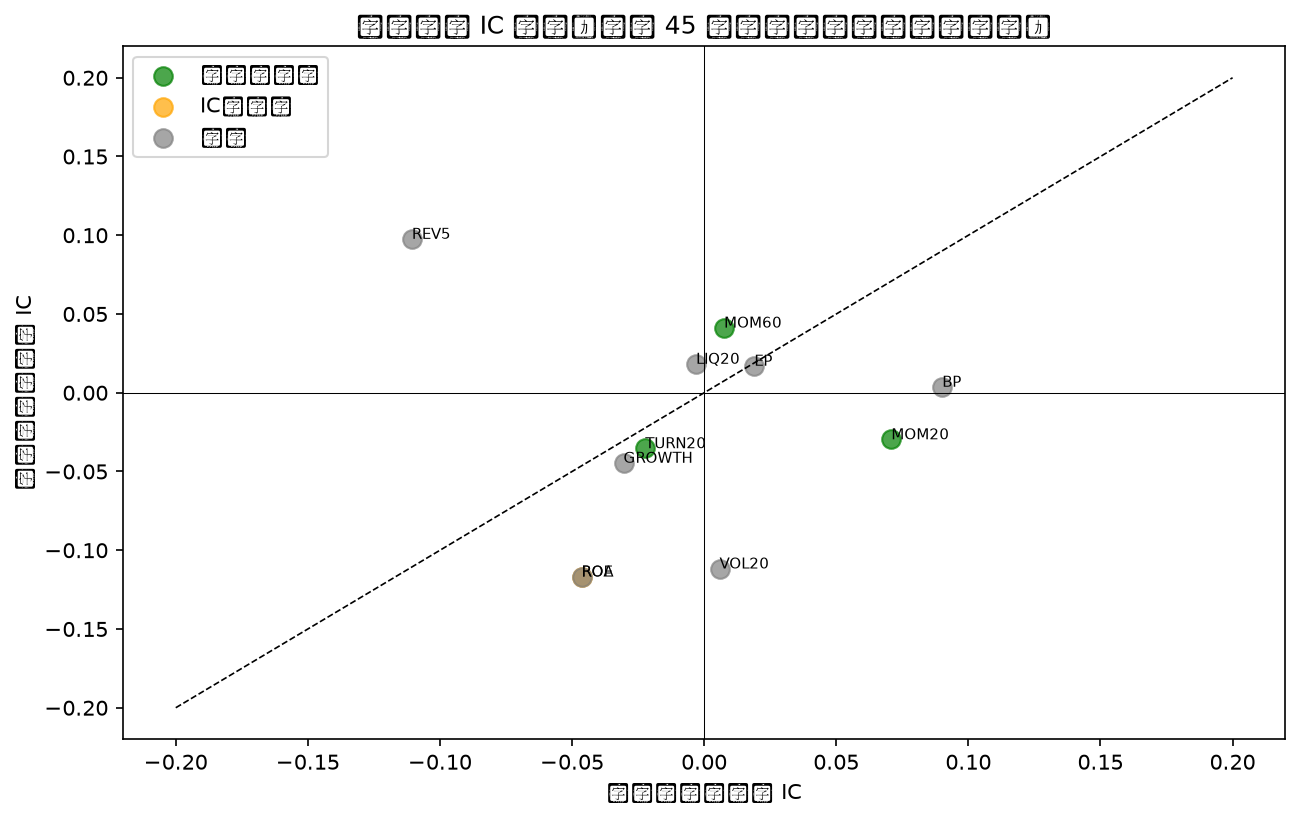
\includegraphics[width=0.95\textwidth]{figures/crowding_ic.png}
\caption{Factor crowding vs. IC}
\end{figure}

\section{Portfolio Backtest}
Out-of-sample from 2023--2024, we compare three long-short portfolios: all-factor equal-weight, IC-significant factors, and causal-significant factors. Each selects the top/bottom 30 stocks by score, equal-weighted long and short, with transaction costs.

\begin{figure}[htbp]
\centering
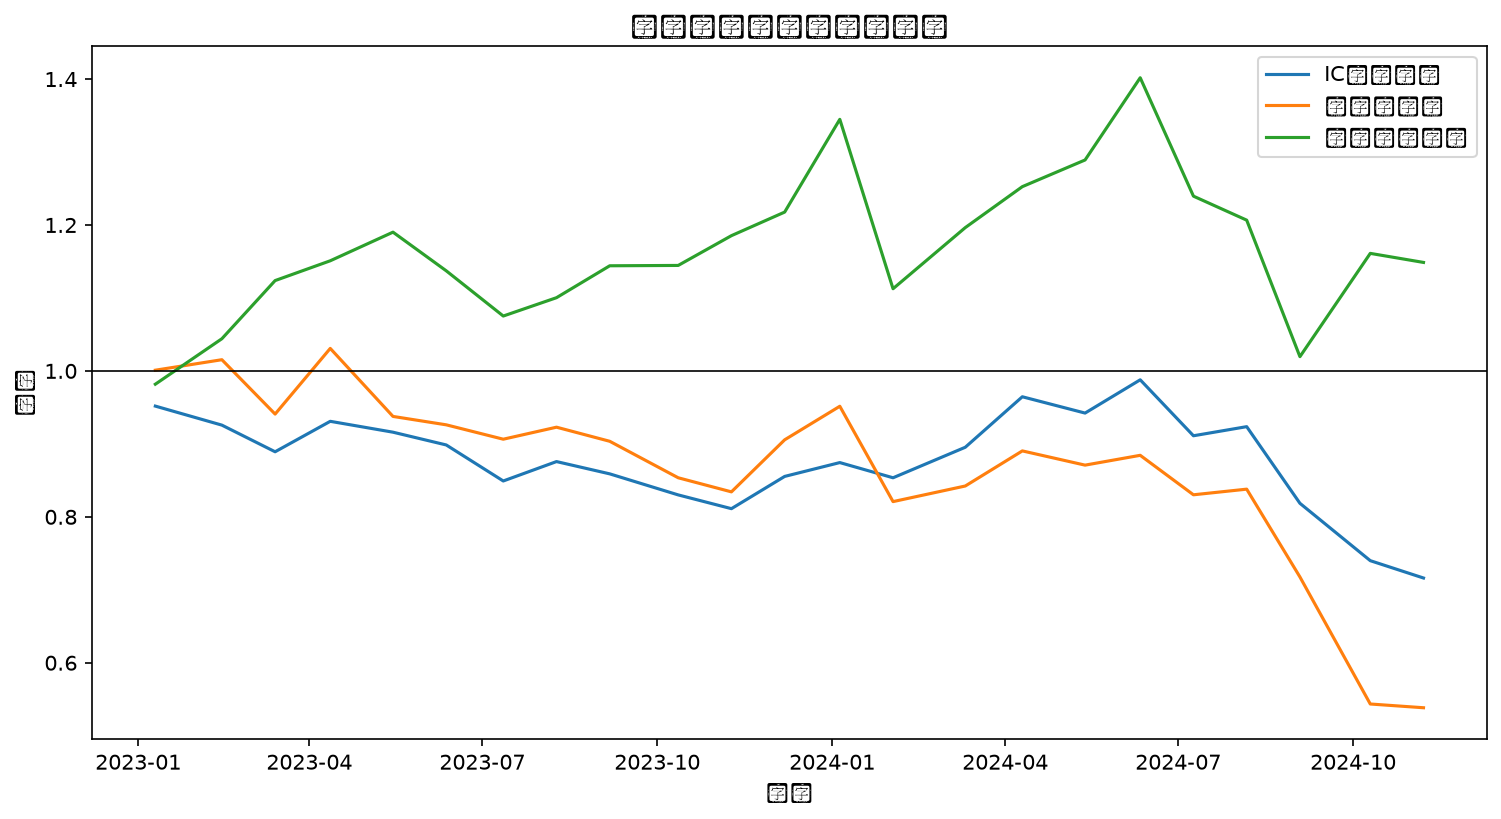
\includegraphics[width=0.95\textwidth]{figures/backtest_nav_curves.png}
\caption{Out-of-sample NAV curves of three portfolios}
\end{figure}

\begin{figure}[htbp]
\centering
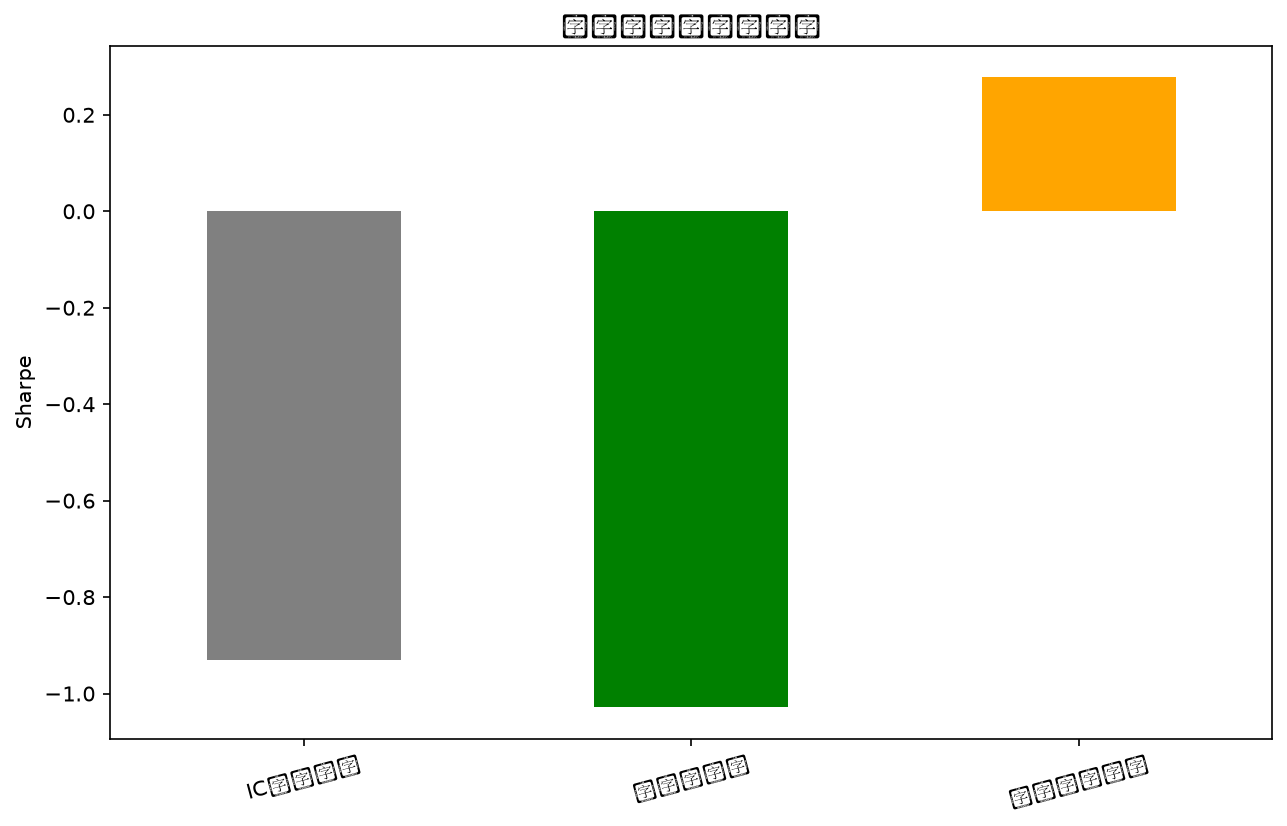
\includegraphics[width=0.95\textwidth]{figures/backtest_sharpe_comparison.png}
\caption{Out-of-sample Sharpe ratio comparison}
\end{figure}

\begin{table}[htbp]
\centering
\caption{Portfolio backtest performance}
\label{tab:backtest}
\begin{tabular}{cccccccccc}
\toprule
组合 & annual\_return & annual\_vol & sharpe & max\_drawdown & win\_rate & total\_return & calmar & information\_ratio & sortino \\ 
\midrule
IC显著因子 & -0.1599 & 0.1719 & -0.9302 & -0.2750 & 0.3478 & -0.2839 & -0.5813 & -0.6407 & -1.5329 \\ 
全因子等权 & -0.2761 & 0.2684 & -1.0286 & -0.4778 & 0.4348 & -0.4617 & -0.5779 & -0.7594 & -1.1583 \\ 
因果显著因子 & 0.0750 & 0.2701 & 0.2777 & -0.2727 & 0.6522 & 0.1487 & 0.2750 & 0.0181 & 0.3383 \\ 
\bottomrule
\end{tabular}
\end{table}

\section{Robustness Checks}
\subsection{Rosenbaum Sensitivity Bounds}
We test robustness to unobserved confounding by varying $\Gamma$ from 1.0 to 2.0. If the effect remains significant at $\Gamma=1.5$, it is moderately robust; at $\Gamma=2.0$, highly robust.

\begin{figure}[htbp]
\centering
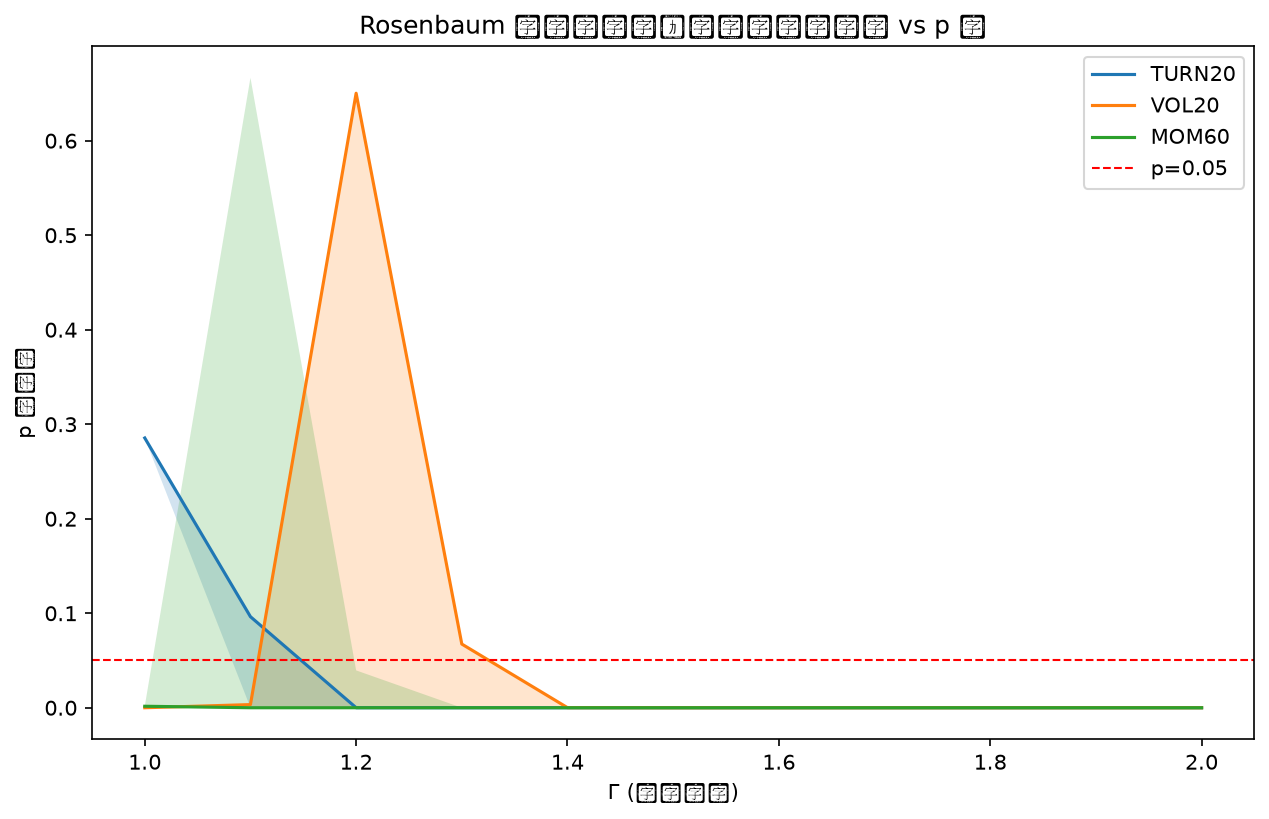
\includegraphics[width=0.95\textwidth]{figures/rosenbaum_bounds.png}
\caption{Rosenbaum sensitivity bounds}
\end{figure}

\subsection{Placebo Tests}
We run the full causal pipeline on random noise factors and cross-sectionally shuffled real factors; the causal effects should be insignificant.

\begin{table}[htbp]
\centering
\caption{Placebo test results}
\label{tab:placebo}
\begin{tabular}{ccccccccc}
\toprule
placebo\_type & method & n\_seeds & n\_sig\_raw & fpr\_raw & n\_sig\_fdr & n\_sig\_valid & binom\_test\_pvalue & fpr\_inflated \\ 
\midrule
noise & CausalForest & 20.0000 & 1.0000 & 0.0500 & 0.0000 & 1.0000 & 0.6415 & 0.0000 \\ 
noise & DML & 20.0000 & 1.0000 & 0.0500 & 0.0000 & 1.0000 & 0.6415 & 0.0000 \\ 
noise & FrontDoor & 20.0000 & 3.0000 & 0.1500 & 0.0000 & 1.0000 & 0.0755 & 0.0000 \\ 
noise & IV & 20.0000 & 2.0000 & 0.1000 & 0.0000 & 1.0000 & 0.2642 & 0.0000 \\ 
shuffled & CausalForest & 20.0000 & 1.0000 & 0.0500 & 0.0000 & 1.0000 & 0.6415 & 0.0000 \\ 
shuffled & DML & 20.0000 & 1.0000 & 0.0500 & 0.0000 & 1.0000 & 0.6415 & 0.0000 \\ 
shuffled & FrontDoor & 20.0000 & 0.0000 & 0.0000 & 0.0000 & 0.0000 & 1.0000 & 0.0000 \\ 
shuffled & IV & 20.0000 & 1.0000 & 0.0500 & 0.0000 & 1.0000 & 0.6415 & 0.0000 \\ 
\bottomrule
\end{tabular}
\end{table}

\subsection{Time-Permutation Test}
We shift the factor forward by one period and estimate its effect on the current-period label. A significant effect would indicate look-ahead bias or spurious time-reversal.

\begin{table}[htbp]
\centering
\caption{Time-permutation test results}
\label{tab:timeperm}
\begin{tabular}{cccc}
\toprule
factor & ate & pvalue & tvalue \\ 
\midrule
EP & -0.0362 & 0.0000 & -5.6947 \\ 
BP & -0.0353 & 0.0000 & -5.6463 \\ 
MOM20 & 0.0945 & 0.0000 & 55.9877 \\ 
MOM60 & 0.0723 & 0.0000 & 23.3189 \\ 
ROE & -0.0053 & 0.3408 & -0.9530 \\ 
ROA & -0.0053 & 0.3408 & -0.9530 \\ 
VOL20 & 0.0343 & 0.0000 & 9.3069 \\ 
TURN20 & 0.0374 & 0.0000 & 9.4091 \\ 
LIQ20 & 0.0040 & 0.3439 & 0.9469 \\ 
GROWTH & 0.0042 & 0.2097 & 1.2549 \\ 
REV5 & -0.0522 & 0.0000 & -19.1234 \\ 
\bottomrule
\end{tabular}
\end{table}

\subsection{Market Regimes}
We split the sample by market trend into bear, neutral, and bull regimes and estimate DML effects separately.

\begin{figure}[htbp]
\centering
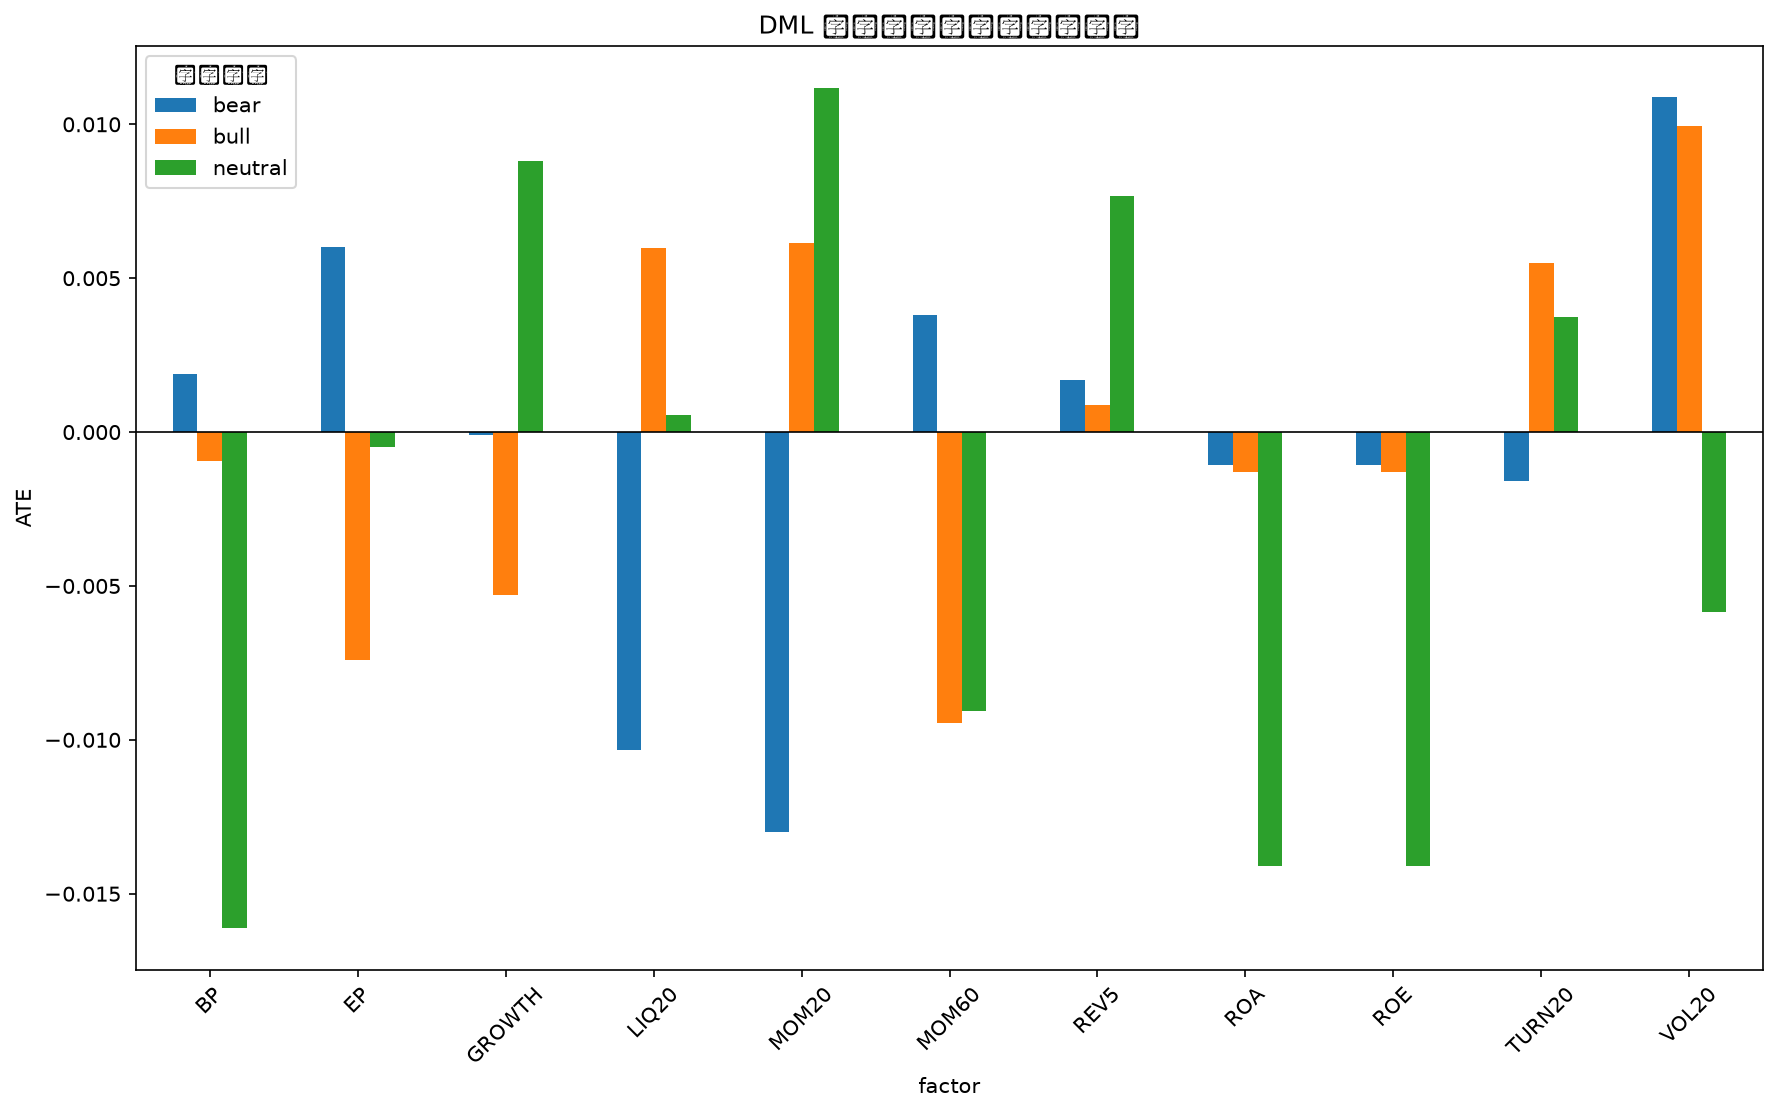
\includegraphics[width=0.95\textwidth]{figures/market_regime_comparison.png}
\caption{DML effects by market regime}
\end{figure}

\section{Math Rigor: do-Calculus and Identification}
\subsection{Back-Door Criterion and do-Calculus}
If a set of controls $Z$ blocks all back-door paths from treatment $D$ to outcome $Y$, then
\begin{equation}
P(Y \mid do(D=d)) = \sum_z P(Y \mid D=d, Z=z) P(Z=z)
\end{equation}

We include industry, size, momentum, and volatility controls for each factor to block back-door paths. The average propensity-score overlap is 0.8852, indicating 良好 common support.

\subsection{Identification Assumptions}
\begin{itemize}
    \item \textbf{Ignorability}: Conditional on controls $Z$, treatment assignment (factor exposure) is approximately independent of potential outcomes (future returns). Unobserved market sentiment and macro shocks remain residual confounders.
    \item \textbf{Common support}: Treated and control units overlap in the control space, verified via propensity score distributions.
    \item \textbf{SUTVA}: In cross-sectional factor studies, individual treatment effects are approximately independent, but spillovers may exist within factor portfolios. High SUTVA-risk factors: \texttt{['EP', 'BP', 'MOM20', 'MOM60', 'ROE', 'VOL20', 'TURN20', 'LIQ20', 'REV5']}.
\end{itemize}

\section{Conclusion and Limitations}
Several traditional IC-significant factors (e.g., ROE) are not causally significant, indicating spurious-correlation risk. The causal-significant portfolio outperforms the IC-significant portfolio out-of-sample (Sharpe 0.2777 vs -0.9302), supporting the robustness of causal factors.

Limitations include the untestable exclusion restriction of IVs, the proxy nature of the mediator in front-door adjustment, residual unobserved confounding, and the sensitivity of causal discovery algorithms to distributional assumptions and sample size. Future work could explore larger samples, richer mediators, and dynamic causal graphs.

\bibliographystyle{plain}
\bibliography{references}

\end{document}
